% Appendix: Supplementary Material (cart-to-purchase EDA)
% Paste at the end of paper_2col.tex (after \bibliography{...} / before \end{document}).
% Upload the three PNGs into an Overleaf folder named figures/, or change the paths below.
% Requires: \usepackage{graphicx}  (usually already loaded in 2-col templates)
% Optional: \usepackage{subcaption} if you prefer subfigures instead of stacked figure*.

\appendix
\section*{Appendix: Supplementary Material}
\addcontentsline{toc}{section}{Appendix: Supplementary Material}

This appendix provides supplementary figures for the cart-to-purchase exploratory analysis on the Synerise RecSys~2025 active-user cohort ($K\geq 5$). The analysis is conducted at the unique user--SKU level: a pair converts if a purchase of that SKU occurs strictly after the first add-to-cart. The main text reports the corresponding conversion rates and time-gap statistics; the figures below visualize conversion composition, the lag distribution among converters, and coarse timing buckets.

\begin{figure*}[t]
\centering
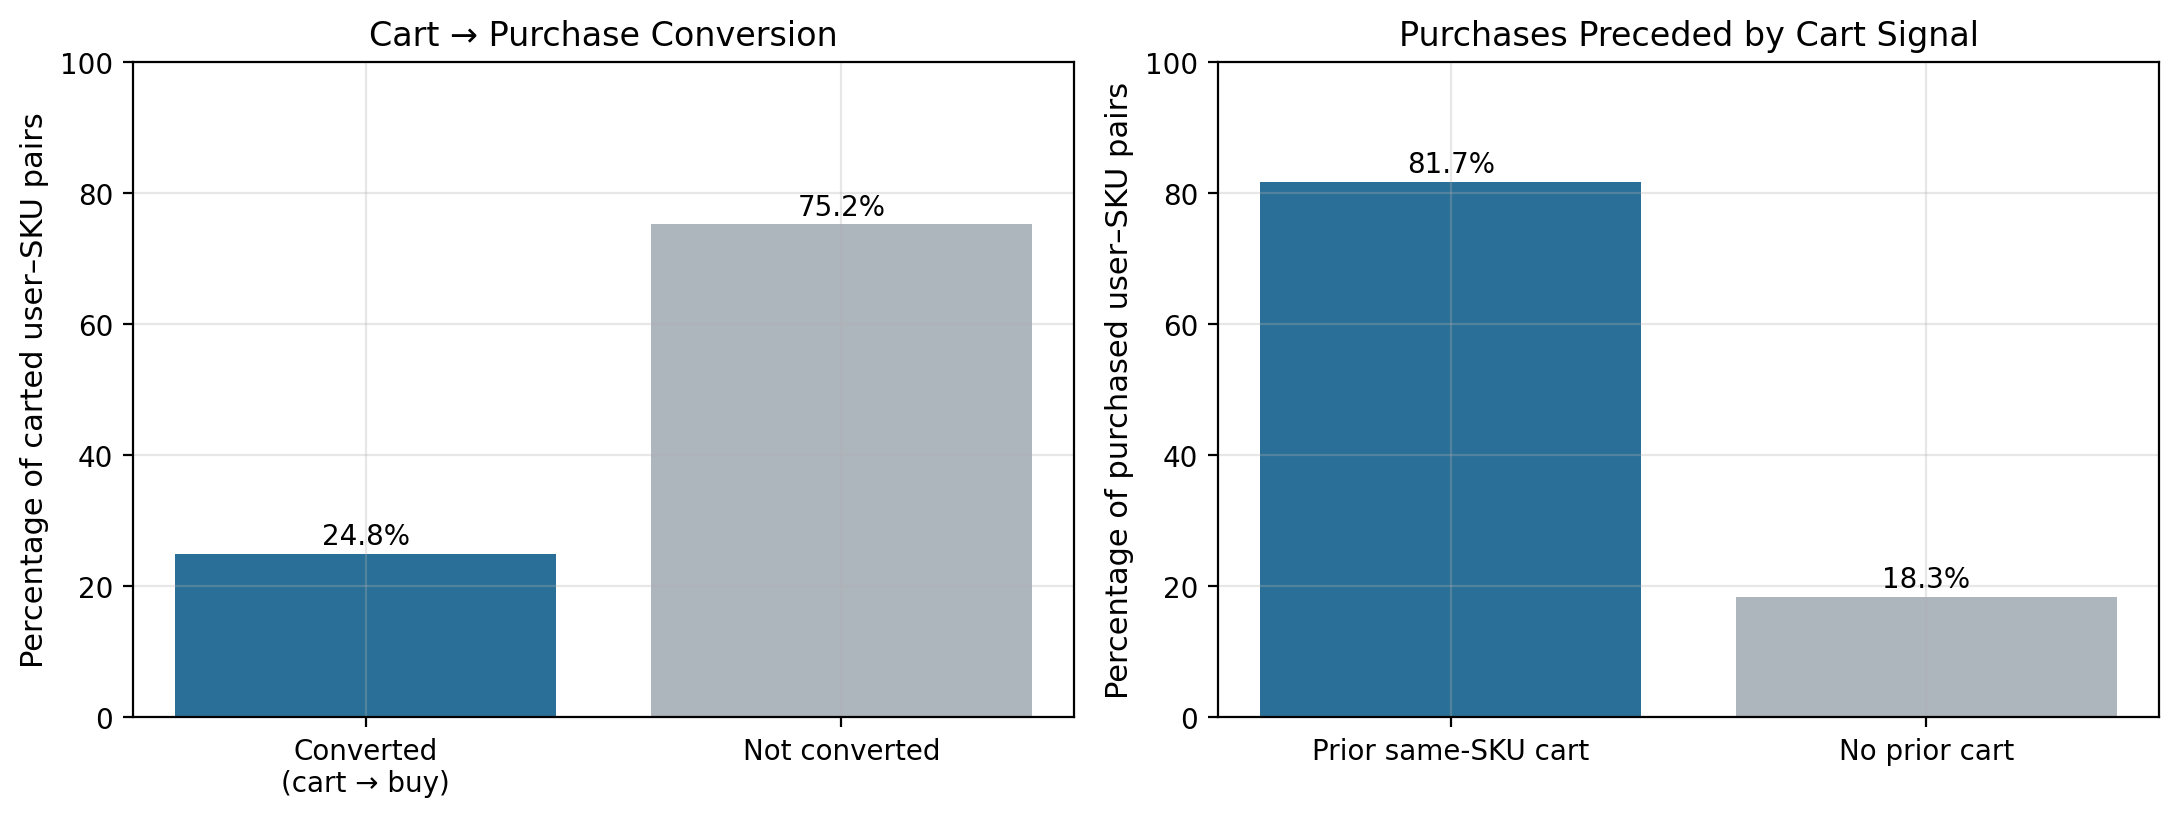
\includegraphics[width=0.92\textwidth]{figures/cart_to_purchase_conversion.png}
\caption{Cart-to-purchase conversion composition on the active-user cohort.
\textbf{Left:} among carted user--SKU pairs, 24.8\% subsequently convert to a purchase of the same SKU and 75.2\% do not.
\textbf{Right:} among purchased user--SKU pairs, 81.7\% were preceded by a same-SKU cart-add, while 18.3\% had no prior cart of that SKU.
Together these panels show that cart activity is both an informative predictor of later purchase and a common precursor of observed purchases.}
\label{fig:app-conversion}
\end{figure*}

\begin{figure*}[t]
\centering
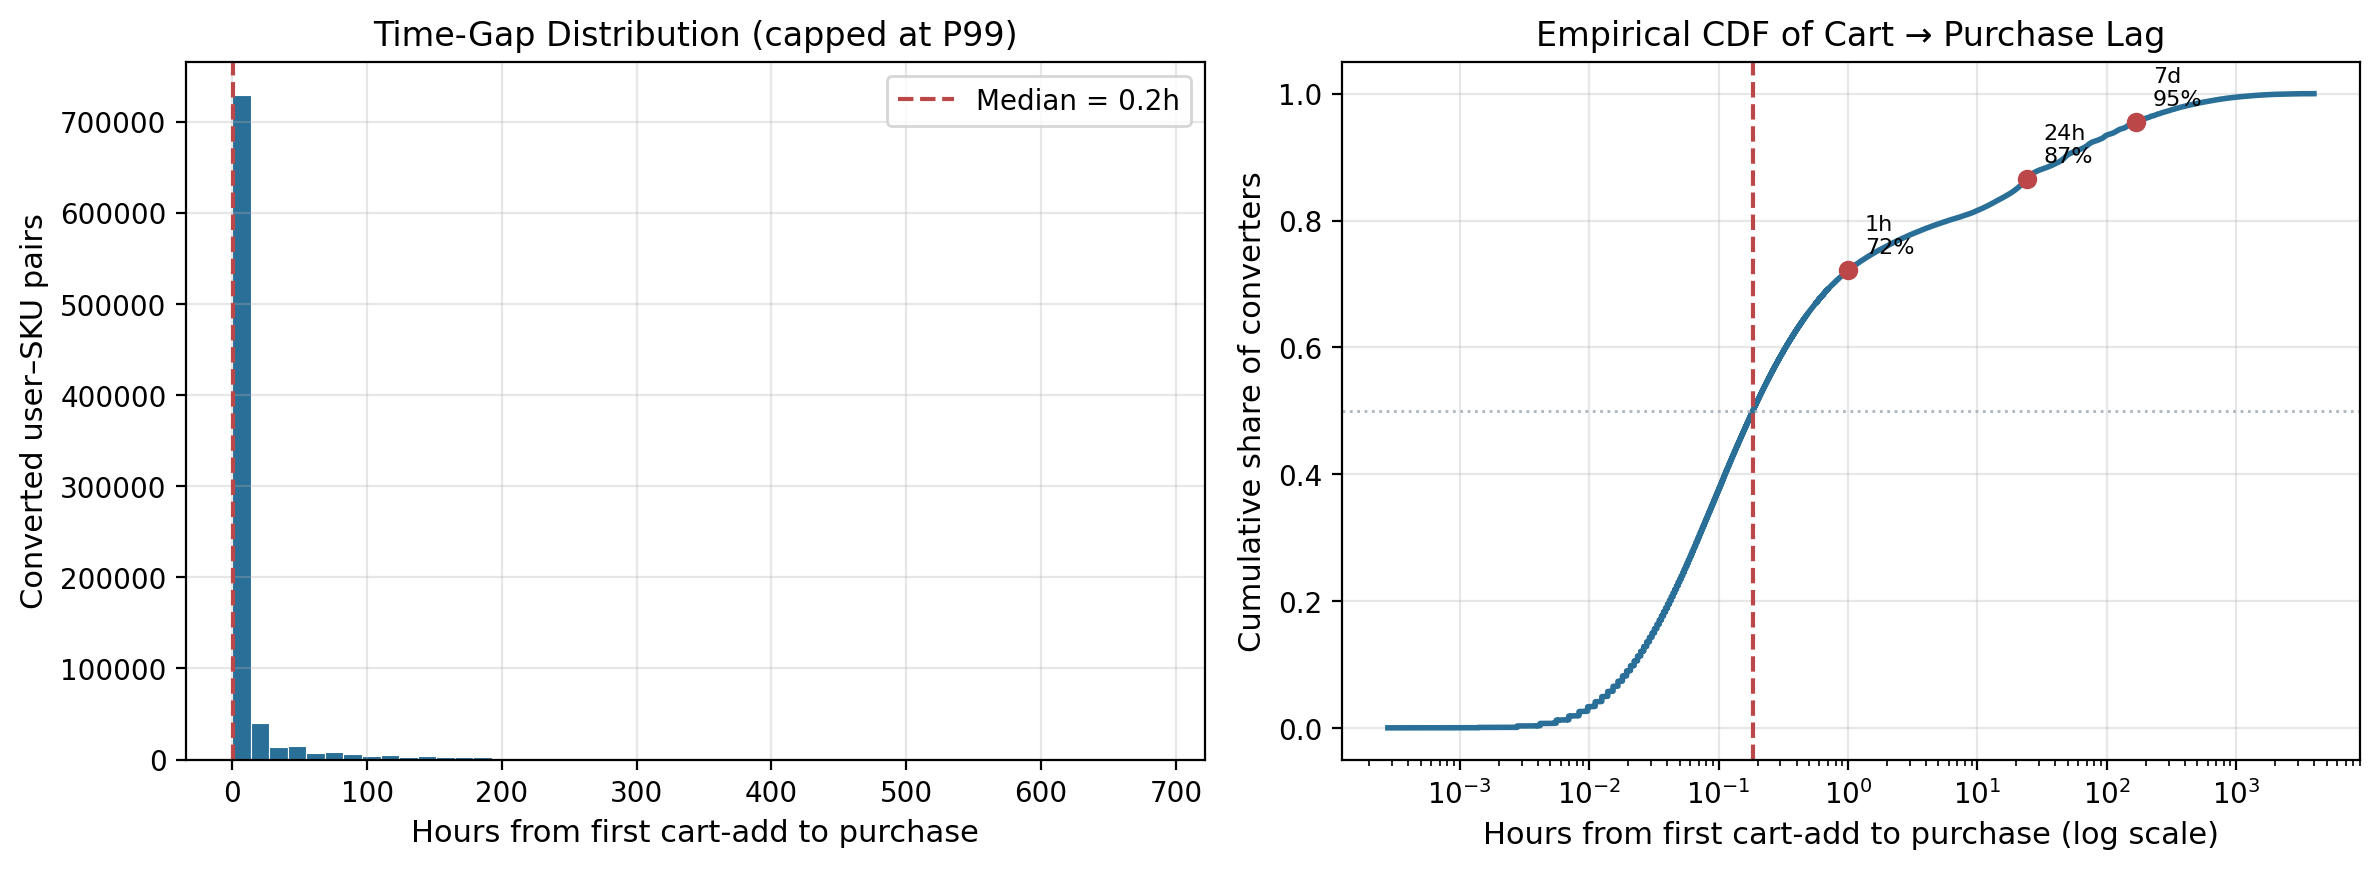
\includegraphics[width=0.92\textwidth]{figures/cart_to_purchase_time_gap.png}
\caption{Time gap from first cart-add to subsequent purchase for converted user--SKU pairs.
\textbf{Left:} histogram of lag in hours (capped at the 99th percentile for readability), with median marked at 0.2~hours ($\approx$11~minutes).
\textbf{Right:} empirical CDF of lag on a log-hour scale, with markers at 1~hour (72\% of converters), 24~hours (87\%), and 7~days (95\%).
The strongly right-skewed distribution indicates that most conversions occur soon after carting, while a long tail accounts for the much larger mean lag.}
\label{fig:app-timegap}
\end{figure*}

\begin{figure*}[t]
\centering
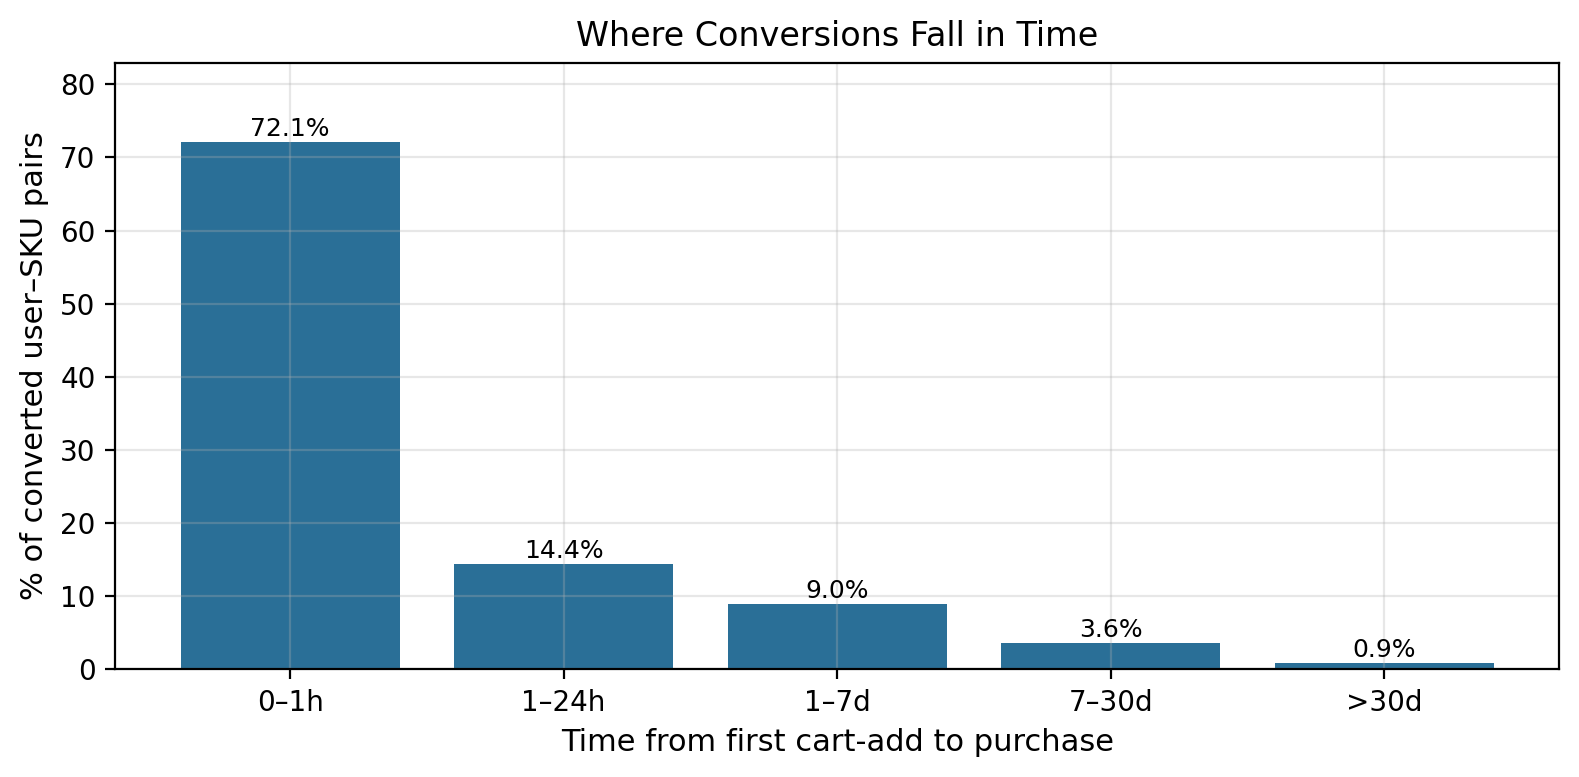
\includegraphics[width=0.72\textwidth]{figures/cart_to_purchase_gap_buckets.png}
\caption{Distribution of converted user--SKU pairs across coarse cart-to-purchase timing buckets.
Of eventual converters, 72.1\% purchase within one hour of the first cart-add, 14.4\% between 1 and 24~hours, 9.0\% between 1 and 7~days, 3.6\% between 7 and 30~days, and 0.9\% after 30~days.
This bucket view reinforces that cart intent is predominantly near-term, which motivates treating recent cart events as fresher signals than sparse historical purchases in sequential recommendation.}
\label{fig:app-buckets}
\end{figure*}
